\usepackage[
    locale=DE 
    separate-uncertainty=true 
    per-mode=symblo-or-fraction
]{siunitx}


\section{Auswertung}
\label{sec:Auswertung}

\subsection{Temperaturverläufe}
%Aufgabenteil a)
\subsection{Temperaturmessung}
Im folgenden Diagramm werden die Verläufe der Temperaturen T1 und T2 in Abhängigkeit der Zeit aufgetragen.
Alle Werte wurden in SI-Einheiten konvertiert.
\begin{figure}
  \centering
  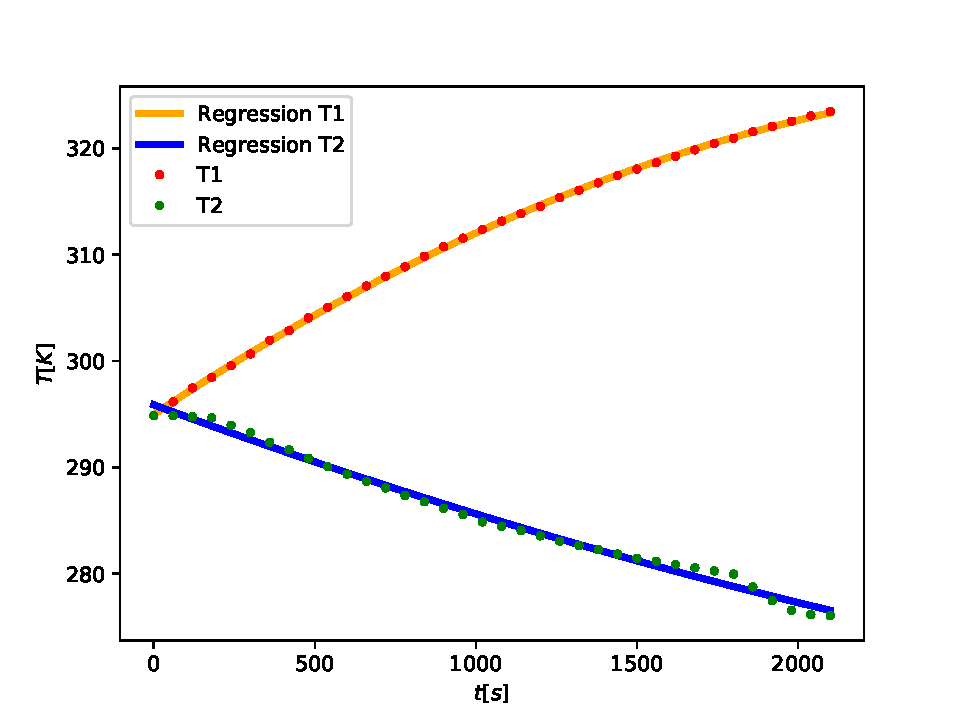
\includegraphics[scale = 0.75]{Temperaturverlaeufe.pdf}
  \caption{Die beiden Temperaturverläufe der Reservoire 1 und 2.}
  \label{fig:TemperaturverlaufA}
\end{figure}
Die eingezeichneten Regressionen sind quadratisch. Ihre Funktionsgleichung lautet:
\begin{equation}
    T(t)=A*t^2+B*t+C
\end{equation}
Dabei sind die Parameter A, B und C:
T1)
$A=\SI{(-3.22491 \pm 0.00419)e(-6)}{\Kelvin\per\second\square}$
$B=\SI{0.02027 \pm 9.11046e(-5)}{\Kelvin\per\second}$
$C=\SI{294.97008 \pm 0.04134}{\Kelvin}$
\\
T2)
$A=\SI{(9.55040 \pm 2.67109)e(-7)}$
$B=\SI{-0.01120 \pm 5.80315e(-4)}$
$C=\SI{295.870187 \pm 0.26336}$

%Aufgabenteil b)
\subsection{Bestimmung der Näherungsfunktion}
Die nicht-linearen Ausgleichsrechnungen sind ebenfalls in \ref{fig:TemperaturverlaufA} skizziert. Der gewählte Ansatz ist
\begin{equation}
  T(t) = \symup{A} \cdot t^2 + \symup{B} \cdot t + \symup{C}.
  \label{eq:Regressionsgleichung}
\end{equation}
\begin{table}
  \centering
  \caption{Parameter der nicht-linearen Ausgleichsrechnung}
  \label{tab:regression1}
  \sisetup{table-format=3.8}
  \begin{tabular}{c S S S S S S}
    \toprule
     {$T$} & {$A [K/s^2]$} & {$\increment A [K/s^2]$} & {$B [K/s]$} & {$\increment B [K/s]$} & {$C [K]$} & {$\increment C [K]$} \\
    \midrule
    {$T_\text{1}$} & 3.2249e-6 &  $\pm$4.1934e-8 &  0.02027984 & $\pm$9.11047e-5 & 294.97008 & $\pm$0.04134 \\
    {$T_\text{2}$} & 0.9550e-6 &  $\pm$26.711e-8 & -0.01120872 & $\pm$58.0316e-5 & 295.87019 & $\pm$0.26336 \\
    
      \bottomrule
  \end{tabular}
\end{table}

%Aufgabenteil c)
\subsection{Bestimmung der Differentailquotienten}
Die Differentailquotienten der Regressionen berechnet man durch einfaches Ableiten der Gleichung \eqref{eq:Regressionsgleichung}.
Nach den Ableitungsregeln ergibt sich:
\begin{equation}
    T(t) = 2\symup{A} \cdot t + \symup{B}
    \label{eq:Regressionableitung}
  \end{equation}
  Nun werden konkrete Werte für 4 verschiedene Temperaturen berechnet werden. Diese sind in unserem Fall die Temperaturen bei 
  den Zeiten $60s, 660s, 1 260s, 1 860s$.
  \begin{table}
    \centering
    \caption{Differentailquotienten}
    \label{tab:Differentailquotienten}
    \sisetup{table-format=3.8}
    \begin{tabular}{c S S S S S S}
      \toprule
       {$T$} & {$A [K/s^2]$} & {$\increment A [K/s^2]$} & {$B [K/s]$} & {$\increment B [K/s]$} & {$C [K]$} & {$\increment C [K]$} \\
      \midrule
      {$T_\text{1}$} & 3.2249e-6 &  $\pm$4.1934e-8 &  0.02027984 & $\pm$9.11047e-5 & 294.97008 & $\pm$0.04134 \\
      {$T_\text{2}$} & 0.9550e-6 &  $\pm$26.711e-8 & -0.01120872 & $\pm$58.0316e-5 & 295.87019 & $\pm$0.26336 \\
      
        \bottomrule
    \end{tabular}
  \end{table}